\section{Introduction to transformers}\label{sec:transformers}

One of the most important innovations in the modern Machine Learning world is undoubtedly the advent of Transformers. Architectures like ChatGPT, Gemini, and a myriad of other AIs are completely revolutionizing the technological landscape. In fact, if you ask experts, this architecture has changed the field of machine learning just as profoundly as the invention of the transistor changed microelectronics! 

\subsection{The Attention Mechanism}

The core idea behind Transformers is relatively simple and originates from Natural Language Processing (NLP). Imagine a simple task: we want to guess the missing word in the middle of a sentence using an ML algorithm. As we previously discussed, a sentence is essentially a sequence of words, making it natural to think that this problem could be solved by a Recurrent Neural Network (RNN). However, we also know the severe limitations of those algorithms, with the vanishing or exploding gradient problem being the primary bottleneck.

An idea that could be far more efficient is to stop processing words sequentially. Instead, we can place them in a matrix, where both the rows and the columns correspond to the words in the sentence. Each entry in this matrix is a number (from 0 to 1) representing the correlation or importance between two words. Superfluous information gets an entry of 0, while highly relevant connections get an entry closer to 1. 

Given the natural mathematical equivalence between matrices and graphs, we can view this sentence as a fully connected graph. Every word is a node, and every connection (matrix entry) is an edge assigned a specific weight $\alpha \in [0,1]$. 

Let us formulate this from a message passing point of view. In a generic GNN, the message passing is basically an update function. The pooling operation aggregates messages "democratically". We update a node's hidden representation $h_i$ by simply summing the messages from its neighbors $j$ \footnote{This is a simplified version of Eq. \ref{eq:node_update}.}:
\begin{equation}
    h_i' = \phi^v\left(h_i, \sum_j \phi^e(h_i, h_j)\right)
\end{equation}
However, it is intuitive to say that certain messages might be vastly more important than others. We want to generalize this to an \textbf{attentional message passing} by weighting the incoming messages with our factor $w_{ij}$:
\begin{equation}
    h_i' = \phi^v\left(h_i, \sum_j w_{ij}(h_i, h_j) \phi^e(h_j)\right)
\end{equation}
During the message passing step, the pooling operation (the sum in this case) ensures that the most relevant messages (those coming from edges with higher weights) contribute the most to the node's update. This is the so-called \textbf{attention mechanism}, briefly introduced in Sec. \ref{sec:intro_att_mech}.

\subsection{The Key, the Query, and the Value}

We immediately realize that we now allow for a weighting mechanism of the importance of the information to be passed to the receiver node $i$. The overall attention algorithm is based on the definition of these weights $w_{ij}$. But how do we actually find them? We certainly do not know them a priori, so they must be learnable parameters that the neural network automatically optimizes during training via gradient descent. To do this, we introduce three distinct concepts: the \textbf{Key}, the \textbf{Query}, and the \textbf{Value}.

This mechanism inherits its logic directly from how large databases operate. Imagine you are on YouTube and you want to search for videos about cats. You type "cat" into the search bar: your search term is the \textit{query} (the anchor). Meanwhile, all the videos in the database are indexed by a \textit{key} (their metadata or tags). The database computes the similarity between your query and the keys to return the most relevant videos.

In the context of our graph, we translate this process into trainable neural networks:
\begin{itemize}
    \item[-] \textbf{The Query ($\vec{q}_i$)}: This is an encoded message of the \textbf{receiver} node $i$ (the anchor looking for information). It is defined via a neural network $\phi^q$ as $\phi^q(h_i) = \vec{q}_i$.
    \item[-] \textbf{The Key ($\vec{k}_j$)}: This is an encoded message of the \textbf{sender} node $j$ (the database entry). It is defined via a neural network $\phi^k$ as $\phi^k(h_j) = \vec{k}_j$.
\end{itemize}

To find the importance of the message from node $j$ to node $i$, we compute the scalar product between the query and the key:
\begin{equation}
    w_{ij} = \vec{k}_j \cdot \vec{q}_i
\end{equation}
This dot product expresses the similarity between the two vectors in the hidden space. During training, the query and key networks will change their weights until the representations of important messages become similar (meaning their scalar product will be large). 

However, this scalar product can theoretically output any real number from $-\infty$ to $+\infty$. If node $i$ receives messages from multiple neighbors, we intuitively want these weights to act as probabilities, meaning they must be bounded between 0 and 1, and their total sum must equal  1. 
We already mentioned another ML context where we take raw real numbers ranging from $-\infty$ to $+\infty$ and normalize them so they sum to 1: multi-class classification! Just like we do to extract class probabilities, we apply a \textit{softmax} function over all the sending nodes $j \in \mathcal{N}_i$:
\begin{equation}
    \alpha_{ij} = \text{softmax}_j(\vec{k}_j \cdot \vec{q}_i) = \frac{\exp(\vec{k}_j \cdot \vec{q}_i)}{\sum_{l \in \mathcal{N}_i} \exp(\vec{k}_l \cdot \vec{q}_i)}
\end{equation}

Once we have computed this normalized weight, we need the actual information to transmit. We do not just send the raw hidden state; instead, we encode it into a new representation.
\begin{itemize}
    \item[-] \textbf{The Value ($\vec{v}_j$)}: This is the actual message that is sent by node $j$, which will be weighted by $\alpha_{ij}$. It is defined via a neural network $\phi^V$ as $\phi^V(h_j) = \vec{v}_j$. 
\end{itemize}

It becomes clear why this is called the "value" of the message: it is the core information encoded to be transmitted, while the scalar product between the key and the query is strictly used to weight \textit{how much} of this information should be accepted by the receiver.

\subsection{Multi-Head Attention}

Is a single set of weights enough to capture all the complex relationships within a graph or a sequence? Consider our initial sentence example: a text has multiple layers of meaning. One connection between two words might be extremely important grammatically (e.g., a missing word must be a verb for the sentence to make sense), while another connection might carry crucial semantic information (e.g., words like "water" and "pH" sharing a scientific context). 

A single scalar weight $w_{ij}$ cannot easily group and represent all these different levels of information simultaneously. If we forced the network to use only one set of weights, it would end up creating a confusing mix of semantic and grammatical information, diluting the true underlying relationships.

The mechanism described above can be generalized by introducing the concept of the \textbf{number of heads} ($n_h$), which drastically increases the expressive power of the network. Instead of calculating a single set of weights, the so-called \textbf{Multi-Head Attention Mechanism} employs $n_h$ sets of independent encoders ($\phi_k^{(n)}, \phi_q^{(n)}, \phi_V^{(n)}$) for each head $n = 1, \dots, n_h$. 

From a visual perspective, you can imagine adding a Z-axis to our graph, where each head represents a completely independent "track" or "rail" of message passing. Take a look at the simple GNN in figure: a "green" track might autonomously learn to focus strictly on grammar, a "blue" track on semantics, and so on \footnote{Of course, that is just a human-centered view of the mechanisms at hand. What we really want to say is that different types of information are correlated based on many different characteristics, and to represent them all a machine needs more than a single criterion. That does not necessarily mean that the machine knows about semantics and grammar, but it is a good analogy.}. Each head calculates its own queries, keys, and values, and computes its own attention weights in parallel.

\begin{center}
    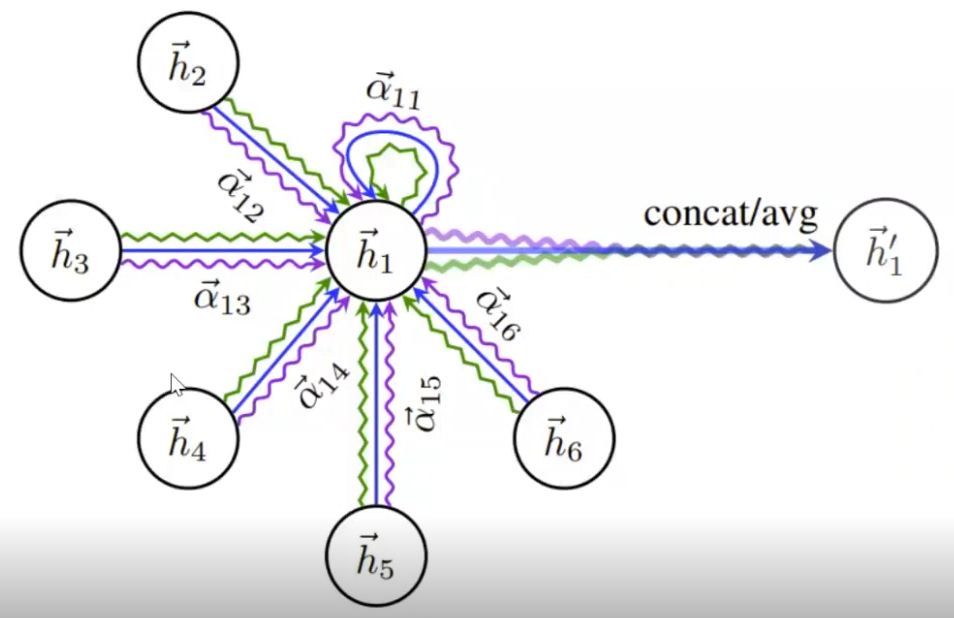
\includegraphics[width=0.5\textwidth]{figuresML_adv/lesson_ml_adv_5_pag_1.png}
\end{center}

Once all these independent tracks have generated their respective output messages, how does the receiving node aggregate them to update its hidden state $h_i'$? If we simply summed or pooled the vectors from the different tracks, we would compress the data and lose the distinct representations the network just worked so hard to separate. 
Therefore, the results are simply \textbf{concatenated} to form a single, massive representation vector. For instance, if we have 3 heads and each outputs a vector of dimension 100, the updated node representation will be a concatenated vector of dimension 300:
\begin{equation*}
    \text{MultiHead} = \text{Concat}(\text{head}_1 \ , \dots, \ \text{head}_{n_h})
\end{equation*}
This resulting vector is finally passed to the node update function $\phi^v$ to produce the new representation $h_i'$. 

The number of heads is a fundamental hyperparameter of the model. It must be chosen and optimized by the user based on the complexity of the specific problem: a value that is too low may fail to capture all necessary correlations, while a value that is too high heavily increases computational cost and the risk of overfitting.

Finally, a quick note on terminology:
\begin{itemize}
    \item[-] \textbf{Self-attention}: This mechanism is often called self-attention when the input nodes pertain to the exact same type (e.g., all words within a single sentence).
    \item[-] \textbf{Cross-attention}: This mechanism is called cross-attention when it operates on different objects or domains (e.g., aligning words in English with words in Italian during a translation task).
\end{itemize}

With all that in mind, we can arrive at our final definition: any neural network architecture that primarily relies on these multi-head attention blocks is referred to as a \textbf{Transformer}. 

Here is a brief recap of what we have said so far: while originally developed for Natural Language Processing, the Transformer treats data not just as a sequence, but as a matrix of correlations and, in this view, every element (or node) can interact with every other element, while the attention mechanism computes a matrix of correlation coefficients. We are now ready for a big computational exercise. 

\section{Hands-on example for Transformers}

Here you will find a complex exercise where we will be building a Transformer from scratch using \texttt{PyTorch}. This is very similar to the exercise about condensation seen in Sec. \ref{sec:GNN_intro}, but you will see the attention mechanism in action. You can access the Notebook at the following link: \url{https://colab.research.google.com/drive/1I8-5t7Ww1-C8c_CDY8ExPbV9vFK-4MOP?usp=sharing}.

Since I have to start a new page in order to input the Notebook in my LaTeX file, here is a list of all the winners of the Gentlemen's Singles Championship at Wimbledon in the Open Era. 

\vspace{5mm}

\begin{tabular}{lllc@{\hspace{3.5em}}lllc}
\textbf{Year} & \textbf{Name} & \textbf{Nat.} & \textbf{\# titles} & \textbf{Year} & \textbf{Name} & \textbf{Nat.} & \textbf{\# titles} \\
1968 & Rod Laver & AUS & 3 & 1998 & Pete Sampras & USA & 5 \\
1969 & Rod Laver & AUS & 4 & 1999 & Pete Sampras & USA & 6 \\
1970 & John Newcombe & AUS & 2 & 2000 & Pete Sampras & USA & 7 \\
1971 & John Newcombe & AUS & 3 & 2001 & Goran Ivanišević & CRO & 1 \\
1972 & Stan Smith & USA & 1 & 2002 & Lleyton Hewitt & AUS & 1 \\
1973 & Jan Kodeš & TCH & 1 & 2003 & Roger Federer & SUI & 1 \\
1974 & Jimmy Connors & USA & 1 & 2004 & Roger Federer & SUI & 2 \\
1975 & Arthur Ashe & USA & 1 & 2005 & Roger Federer & SUI & 3 \\
1976 & Björn Borg & SWE & 1 & 2006 & Roger Federer & SUI & 4 \\
1977 & Björn Borg & SWE & 2 & 2007 & Roger Federer & SUI & 5 \\
1978 & Björn Borg & SWE & 3 & 2008 & Rafael Nadal & ESP & 1 \\
1979 & Björn Borg & SWE & 4 & 2009 & Roger Federer & SUI & 6 \\
1980 & Björn Borg & SWE & 5 & 2010 & Rafael Nadal & ESP & 2 \\
1981 & John McEnroe & USA & 1 & 2011 & Novak Djokovic & SRB & 1 \\
1982 & Jimmy Connors & USA & 2 & 2012 & Roger Federer & SUI & 7 \\
1983 & John McEnroe & USA & 2 & 2013 & Andy Murray & GBR & 1 \\
1984 & John McEnroe & USA & 3 & 2014 & Novak Djokovic & SRB & 2 \\
1985 & Boris Becker & FRG & 1 & 2015 & Novak Djokovic & SRB & 3 \\
1986 & Boris Becker & FRG & 2 & 2016 & Andy Murray & GBR & 2 \\
1987 & Pat Cash & AUS & 1 & \textbf{2017} & \textbf{Roger Federer} & \textbf{SUI} & \textbf{8} \\
1988 & Stefan Edberg & SWE & 1 & 2018 & Novak Djokovic & SRB & 4 \\
1989 & Boris Becker & FRG & 3 & 2019 & Novak Djokovic & SRB & 5 \\
1990 & Stefan Edberg & SWE & 2 & 2020 & \textit{Not held} & - & - \\
1991 & Michael Stich & GER & 1 & 2021 & Novak Djokovic & SRB & 6 \\
1992 & Andre Agassi & USA & 1 & 2022 & Novak Djokovic & SRB & 7 \\
1993 & Pete Sampras & USA & 1 & 2023 & Carlos Alcaraz & ESP & 1 \\
1994 & Pete Sampras & USA & 2 & 2024 & Carlos Alcaraz & ESP & 2 \\
1995 & Pete Sampras & USA & 3 & 2025 & Jannik Sinner & ITA & 1 \\
1996 & Richard Krajicek & NED & 1 & 2026 & Jannik Sinner & ITA & 2 \\
1997 & Pete Sampras & USA & 4 & & & & \\
\end{tabular}


%\includepdf[pages=-, pagecommand={\thispagestyle{plain}}]{lezioni/e_ML_adv_5hands_on.pdf}

% ML_10 nel mio colab